\begin{figure}[ht!]
\centering
  \caption{Silhouette analysis}\label{fig:Silhouette}
   \begin{subfigure}[b]{\textwidth}
   \centering
   \caption{Average silhouette width for different numbers of clusters \textit{k}} \label{fig:G3_silhouette_2}
   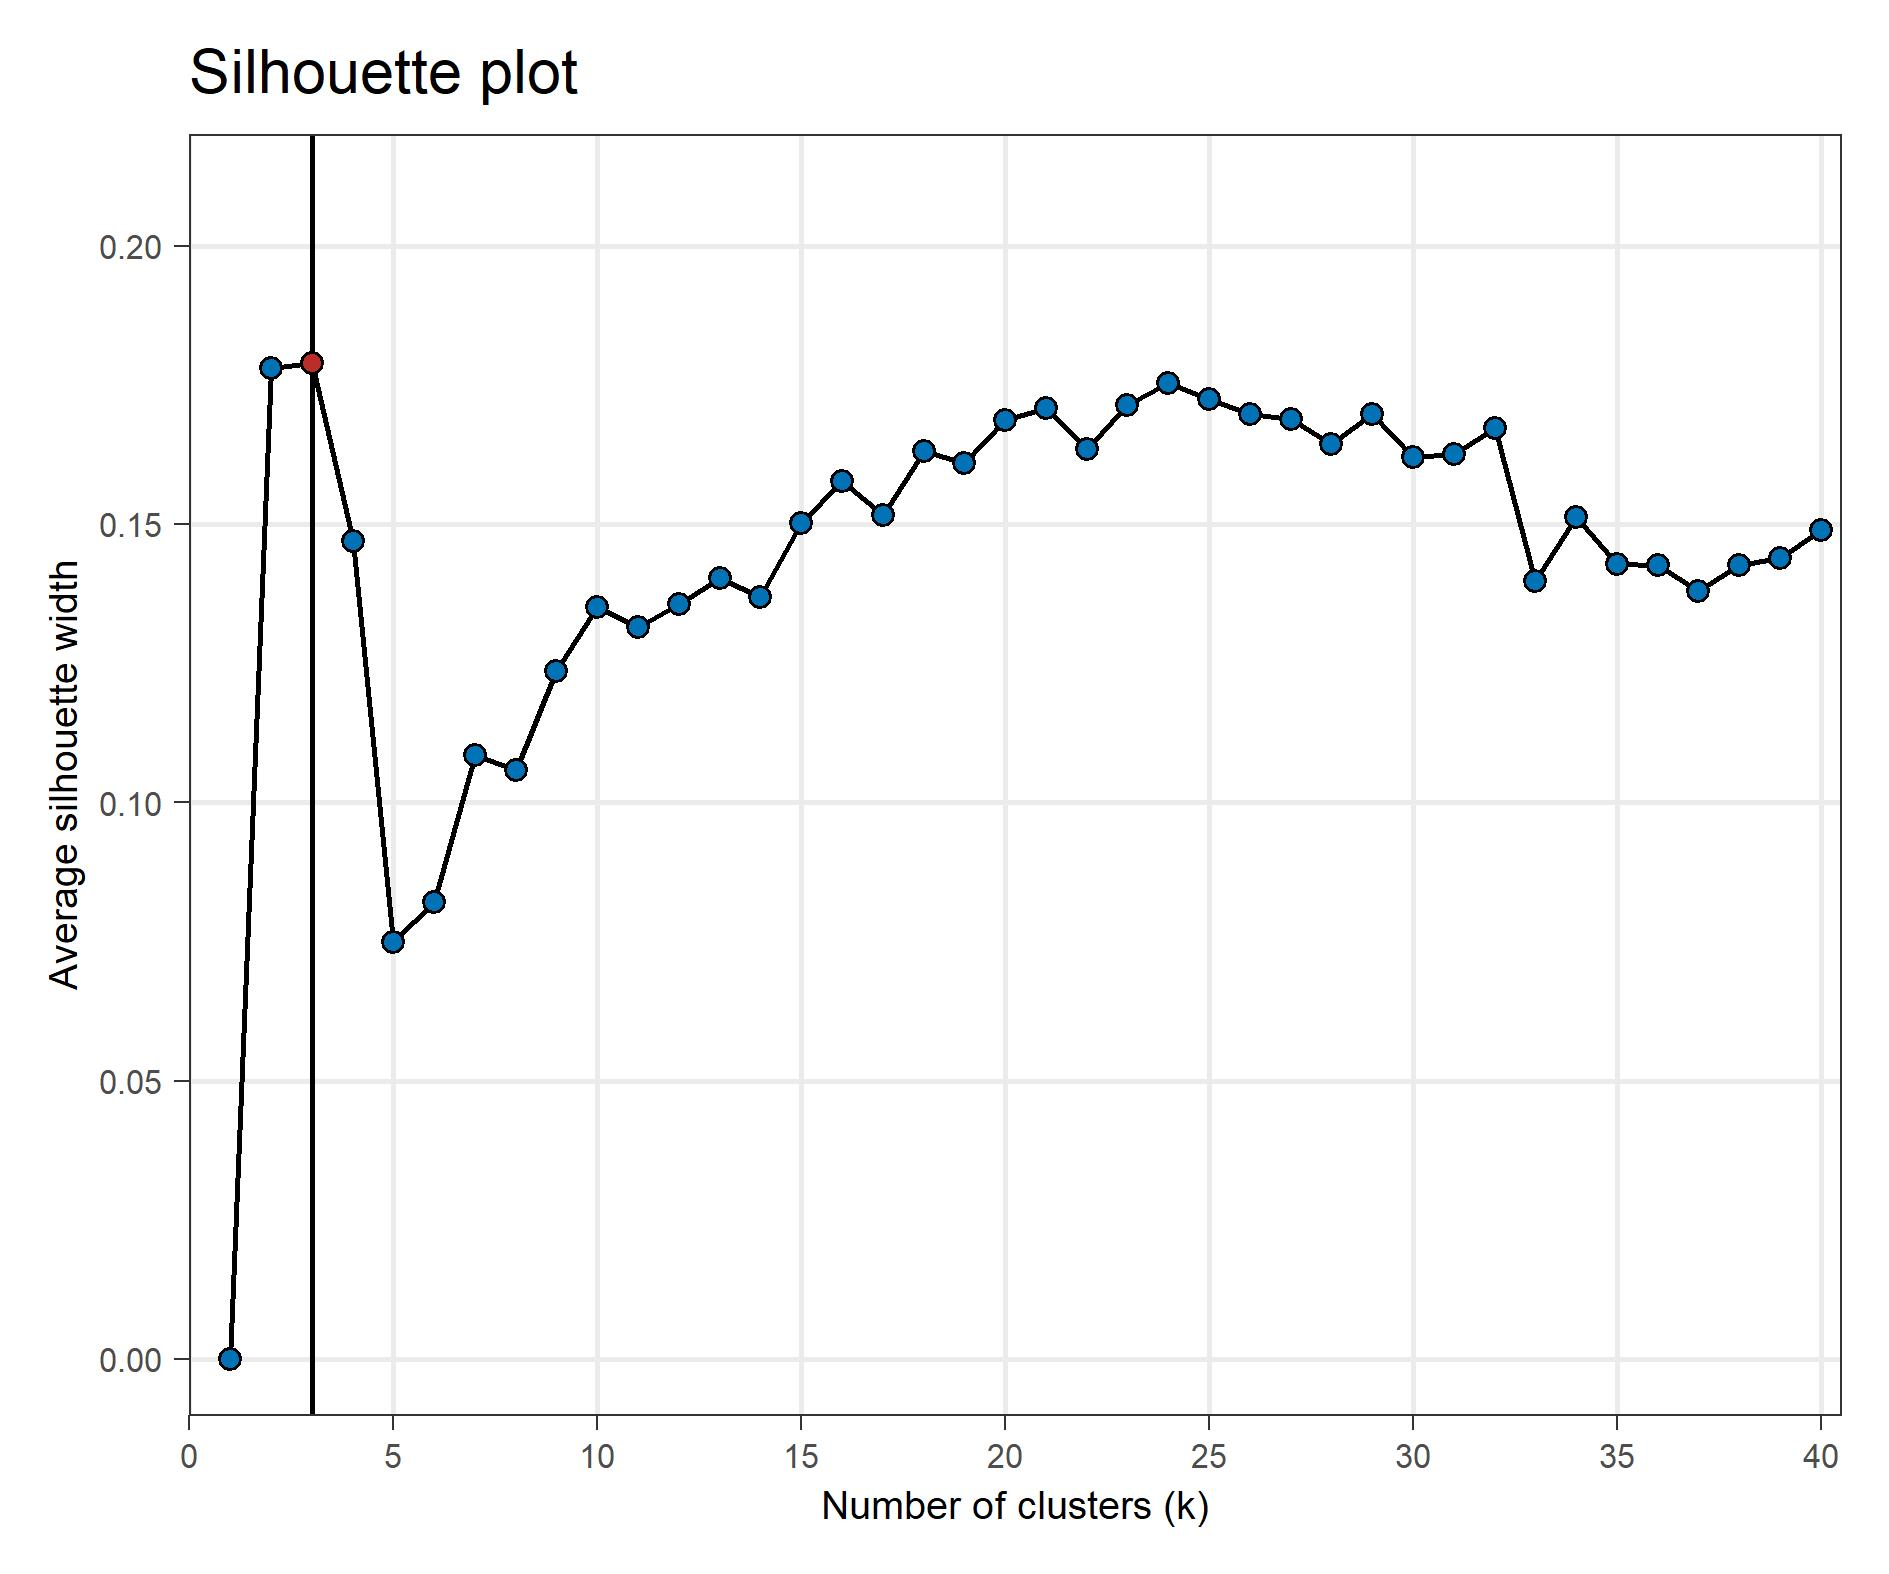
\includegraphics{Figures_Appendix/Figure_Silhouette_2}
   \begin{subcaption2}
     This figure displays the average silhouette width across all clusters for different numbers of clusters \textit{k}. We perform k-means clustering on a dataset with 87 country-level observations. Observations include information on vertical and horizontal distribution, average carbon intensity and \textit{adjusted} feature importance, i.e., we adjust feature importance for country-level model performance. Vertical line and red point indicate the number of clusters that maximizes average silhouette width across all clusters.
   \end{subcaption2}
   \end{subfigure}
 \end{figure}
 \clearpage

 \begin{figure}[ht!]\ContinuedFloat
   \centering
   \begin{subfigure}[b]{\textwidth}
   \centering
    \caption{Average silhouette width for each country per cluster \textit{k}} \label{fig:G4_silhouette_2}
   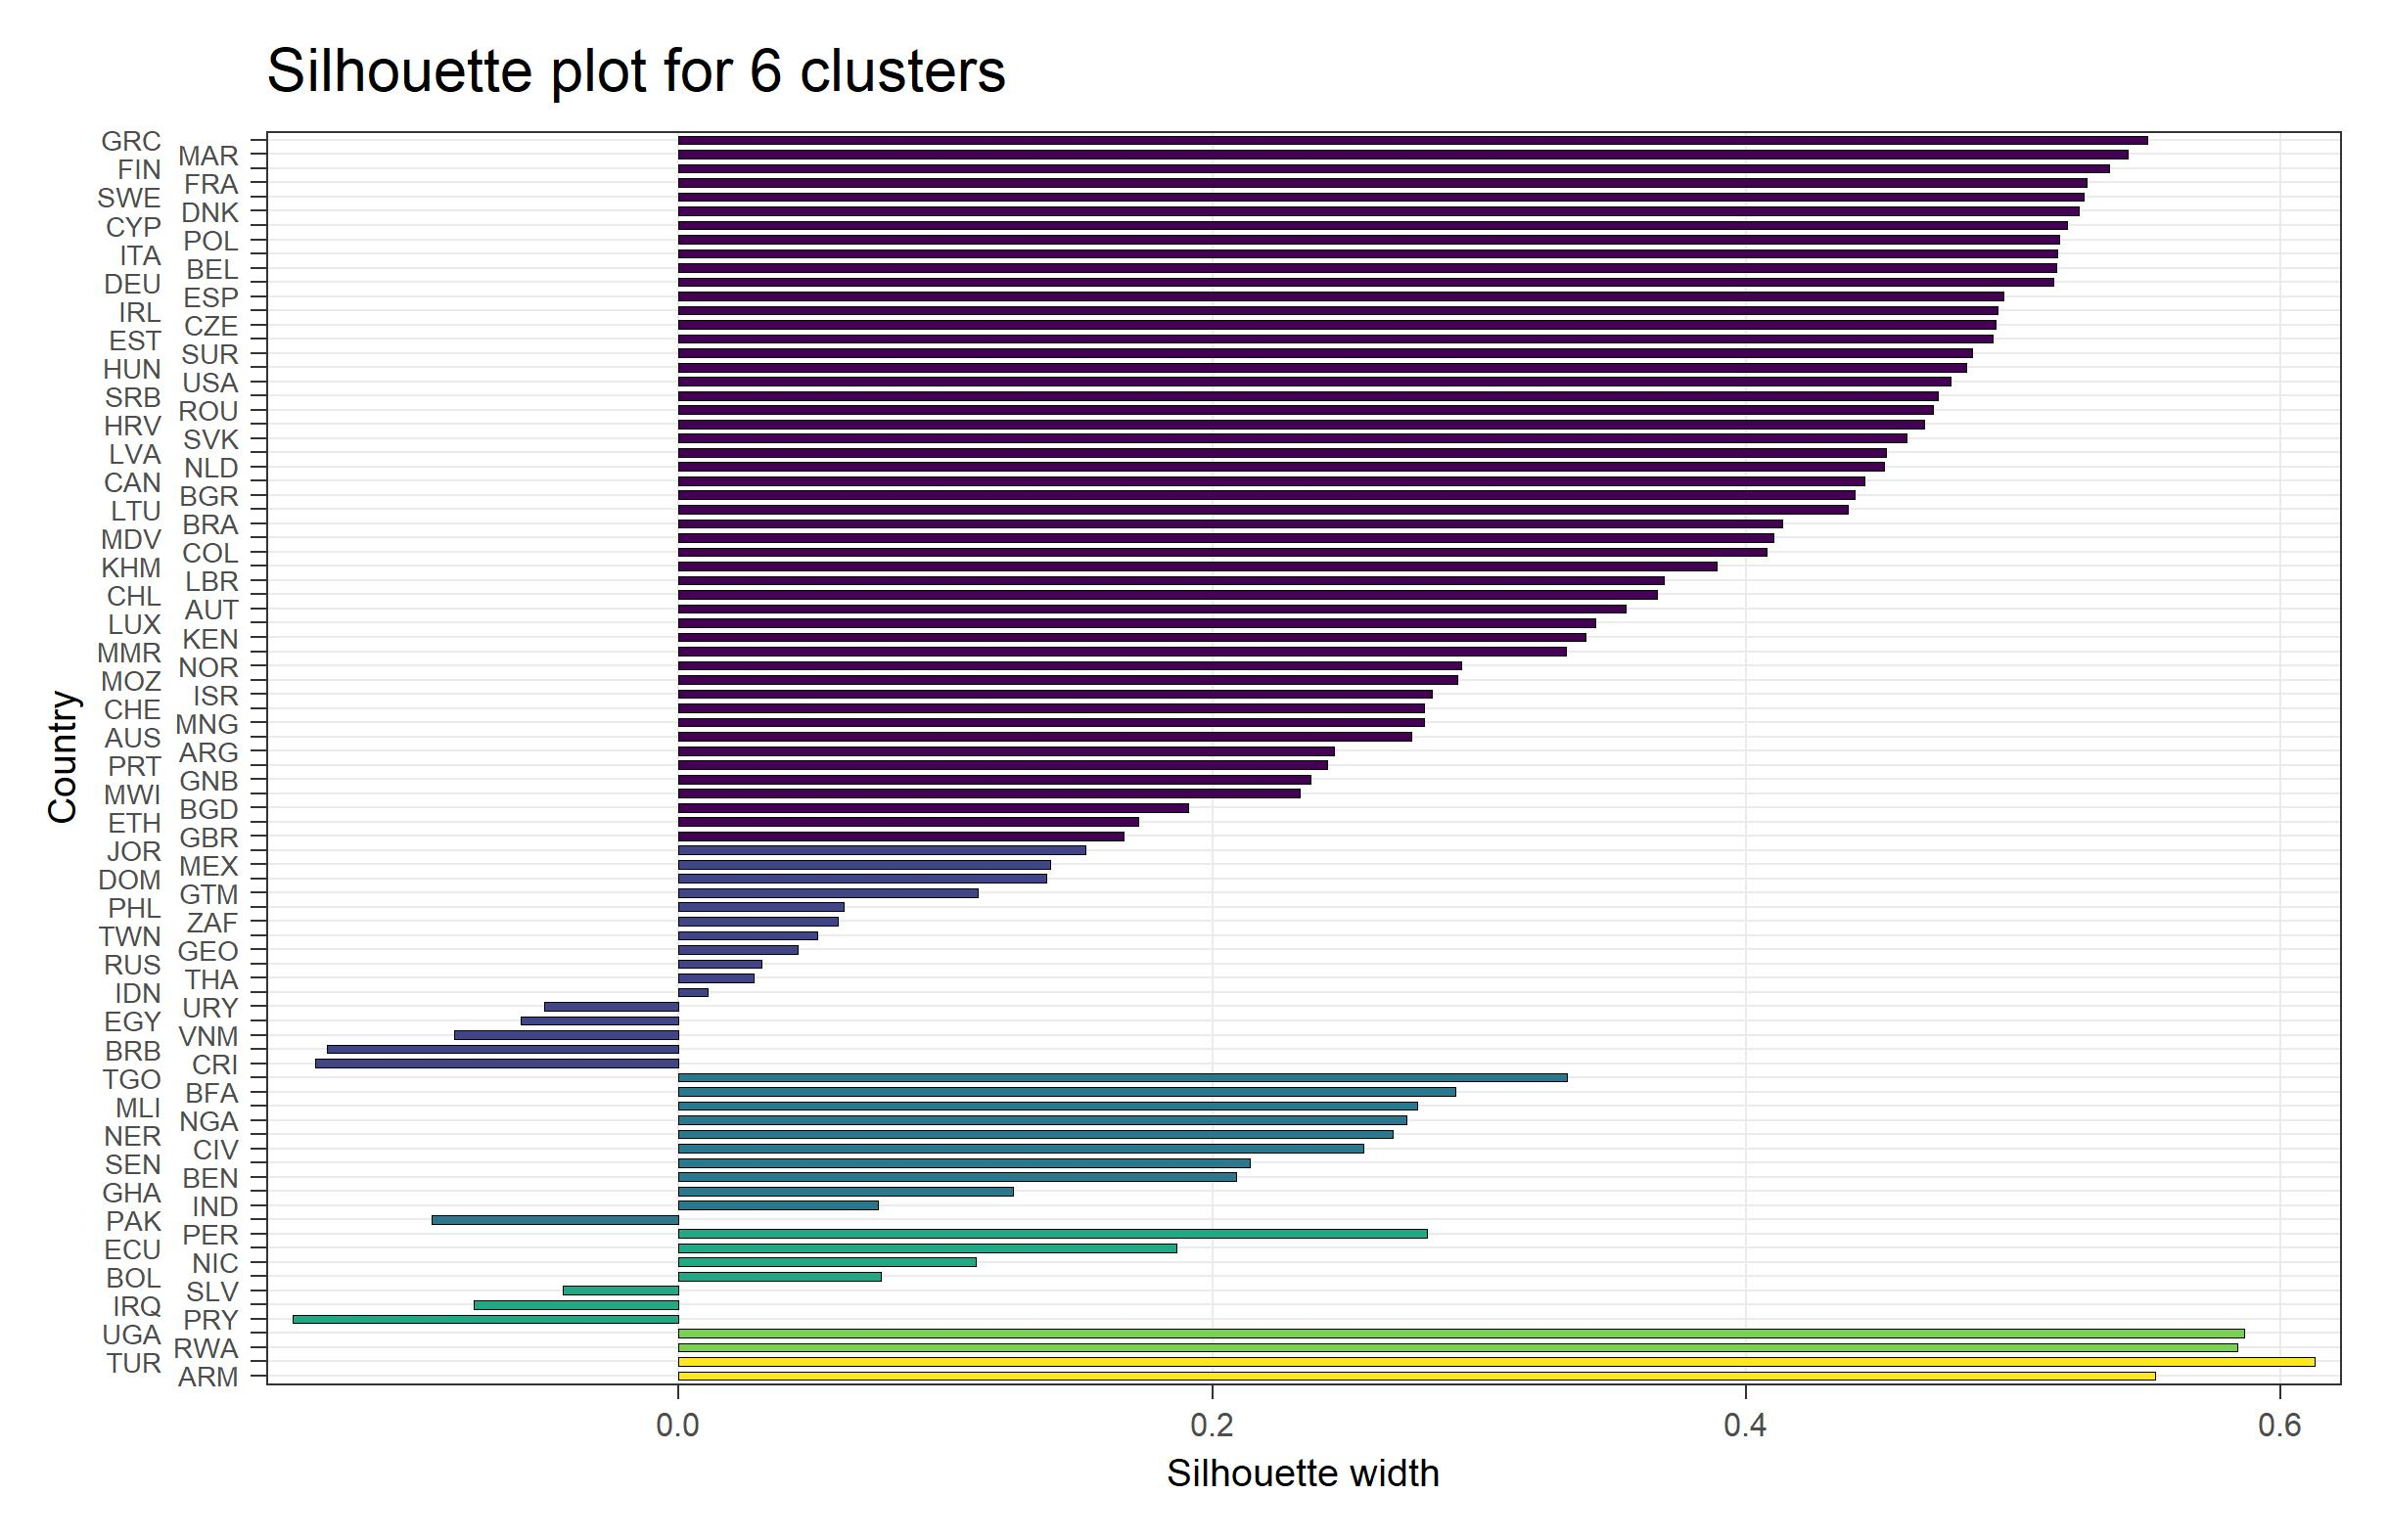
\includegraphics{Figures_Appendix/Figure_Silhouette_Clusters_2}
   \begin{subcaption2}
     This figure displays the silhouette for each country for six clusters. We perform k-means clustering on a dataset with 87 country-level observations. Observations include information on vertical and horizontal distribution, average carbon intensity and \textit{adjusted} feature importance, i.e. we adjust feature importance for country-level model performance. We order observations (y-axis) by clusters with most observations and by silhouette width. Silhouette width expresses how well each observation fits in its cluster, also in comparison to the observations from the least distant, but different cluster.
   \end{subcaption2}
   \end{subfigure}
 \end{figure}
 \clearpage

\begin{figure}[ht!]\ContinuedFloat
   \centering
   \begin{subfigure}[b]{\textwidth}
   \centering
   \caption{Average silhouette width for different numbers of clusters \textit{k}} \label{fig:G1_silhouette}
   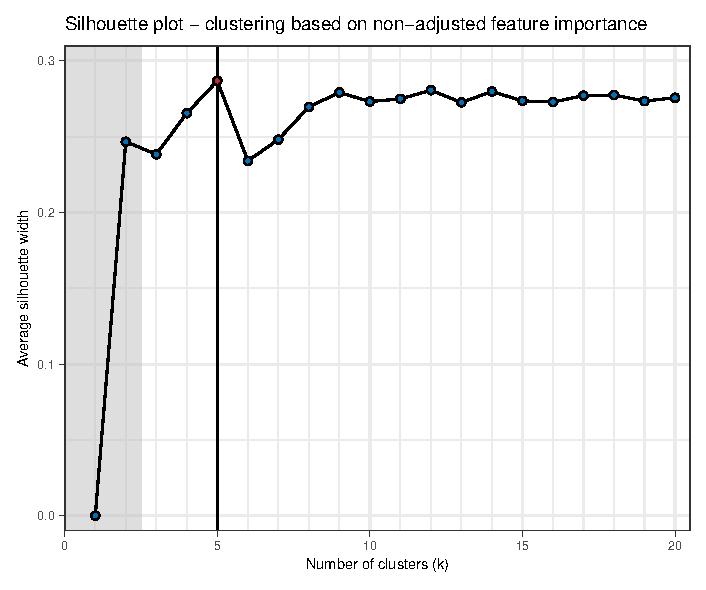
\includegraphics{Figures_Appendix/Figure_Silhouette_1}
   \begin{subcaption2}
     This figure displays the average silhouette width across all clusters for different numbers of clusters \textit{k}. We perform k-means clustering on a dataset with 87 country-level observations. Observations include information on vertical and horizontal distribution, average carbon intensity and feature importance. In contrast to Figure \subref{fig:G3_silhouette_2}, we do not adjust feature importance for country-level model performance. Vertical line and red point indicate the number of clusters that maximizes average silhouette width across all clusters.
   \end{subcaption2}
   \end{subfigure}
 \end{figure}

 \clearpage

 \begin{figure}[ht!]\ContinuedFloat
   \centering
   \begin{subfigure}[b]{\textwidth}
   \centering
   \caption{Average silhouette width for each country per cluster \textit{k}} \label{fig:G2_silhouette}
   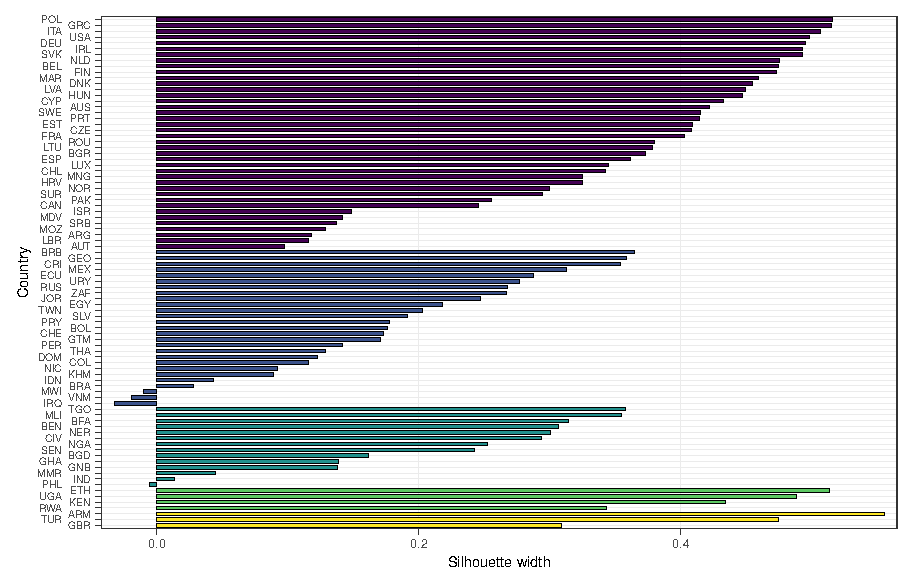
\includegraphics{Figures_Appendix/Figure_Silhouette_Clusters_1}
   \begin{subcaption2}
     This figure displays the silhouette for each country for 13 clusters. We perform k-means clustering on a dataset with 87 country-level observations. Observations include information on vertical and horizontal distribution, average carbon intensity and feature importance. In contrast to Figure \subref{fig:G2_silhouette}, we do not adjust feature importance for country-level model performance. We order observations (y-axis) by clusters with most observations and by silhouette width. Silhouette width expresses how well each observation fits in its cluster, also in comparison to the observations from the least distant, but different cluster.
   \end{subcaption2}
   \end{subfigure}
 \end{figure}
 \clearpage